
\section{NP-Hard Problems Considered} \label{sec:problem}
    \subsection{Maximum Cut (Max-Cut)}
        The maximum cut (max-cut) problem is a decision problem known to be NP-complete \cite{karp2010reducibility}. Given an undirected graph and an integer $k$, the cut problem determines whether there is a partition of the nodes into two complementary subsets such that the number of edges between the two subsets is at least $k$. A \emph{maximum cut} is a cut that is as large as any cut for that graph. Figure \ref{fig:maxcut} shows a maximum cut for an example graph.

        The optimisation version of this problem is NP-hard which aims to maximise the sum of the weights of the edges in the cut. Let $G=(V,E)$ be a weighted, undirected $n$-graph with edge weights $w_{uv}>0$, $w_{uv}=w_{vu}$ for all $(u,v)\in E$. For each node $u$, we assign $x_u=\pm1$ to separate the nodes into the two complementary subsets. The max-cut problem can then be formulated as a binary quadratic program of the form 
        \begin{align}
        \begin{split}
            &\text{maximise} \quad  C_{MC}=\frac{1}{2}\sum_{(u,v)\in E}w_{uv}(1-x_ux_v) \\
            &\text{subject to} \quad\quad x_u\in\{-1,1\}\quad\forall u\in V.
        \end{split}
        \end{align}
        Equivalently, we can formulate the max-cut problem as an Ising spin glass model  through the trivial mapping $x_u\mapsto s_u$, where $s_u\in\{-1,1\}$. We then obtain the Ising energy function for the max-cut problem given by
        \begin{align}
            \begin{split}
                H(s_1,\dots,s_n) &= \frac{1}{2}\sum_{(u,v)\in E} w_{uv}(1-s_us_v) \\
                &=\sum_{u<v}\frac{w_{uv}}{2} - \sum_{u<v}\frac{w_{uv}}{2}s_us_v.
            \end{split}
        \end{align}
        Setting $J_{uv}:= w_{uv}/2$ gives an Ising energy function that satisfies \eqref{eq:ising} up to a constant. Finally, promoting the spin variables to Pauli-$Z$ spin matrices $s_u\mapsto\sigma_u^z$ gives a cost Hamiltonian $H_{MC}$ in the form of \eqref{eq:ising_quantum}, which returns
        \begin{equation}
            H_{MC} = -\sum_{u<v}\frac{w_{uv}}{2}\sigma^z_u\sigma^z_v+\sum_{u<v}\frac{w_{uv}}{2}.
        \end{equation}

        \begin{figure}[H]

            \begin{center}
                %\begin{tikzpicture}
                %    \begin{scope}[every node/.style={circle,thick,draw}]
                %        \node (1) at (-2.5,1.2) {0};
                %        \node (2) at (-1,0) {1};
                %        \node (3) at (1,0) {2};
                %        \node (4) at (-2.3,-1.3) {3};
                %        \node (5) at (2.5,-0.8) {4};
                %        \node (6) at (0,1.5) {5} ;
                %    \end{scope}
                %    \begin{scope}[>={[black]},
                %        every node/.style={fill=white,circle}]
                %        \path [-] (1) edge (2);
                %        \path [-] (4) edge (2);
                %        \path [-] (6) edge (2);
                %        \path [-] (6) edge (3);
                %        \path [-] (2) edge (3);
                %        \path [-] (3) edge (5);
                %    \end{scope}
                %    
                %\end{tikzpicture}
                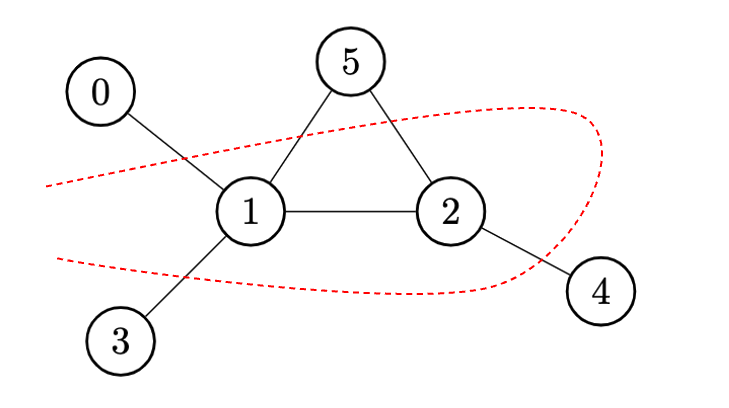
\includegraphics[scale=0.3]{"figures/maxcut.png"}
            \end{center}
            \caption{Unweighted graph with max-cut of 5. The cut can be represented by the disjoint sets $S_1=\{0,3,4,5\}$ and $S_2=\{1,2\}$, which corresponds to a bitstring encoding of $\mathbf{x}=100111$ or $\mathbf{x}=011000$.}
            \label{fig:maxcut}
        \end{figure}

    \subsection{Number Partitioning (NPP)}

        The NPP is another well-known NP-complete problem \cite{karp2010reducibility}. Given a set of integers, the problem is to determine whether there exists a partition of the input set into two subsets, such that the difference between the sums of the two subsets is 0 or 1.

        The optimisation version of this problem is NP-hard which aims to minimise the difference in the sums of the two partitions. A solution is called a perfect partition if the difference is 0 or 1 if the sum of the entire set is even or odd respectively. Let $S=\{n_1,\dots,n_N\}$ be a set of $n$-positive integers. Then, the NPP becomes
        \begin{align}
        \begin{split}
                &\text{minimise} \quad  C_{NPP}=\lr(){\sum_{i=1}^Nn_ix_i}^2 \\
                &\text{subject to} \quad x_i\in\{-1,1\}\quad\forall i\in\{1,\dots,N\}.
        \end{split}
        \end{align}
        Again, we can equivalently formulate NPP as an Ising spin glass model by the trivial mapping $x_i\mapsto s_i$, where $s_i\in\{-1,1\}$. We obtain the Ising energy function for NPP given by 
        \begin{align}
            \begin{split}
                H(s_1,\dots,s_n) &= \lr(){\sum^N_{i=1}n_is_i}^2 \\
                &= 2\sum^N_{i<j} n_in_js_is_j + \sum^N_{i=1}n_i^2.
            \end{split}
        \end{align}
        Setting $J_{ij}:=-2n_in_j$ gives an Ising energy function that satisfies Equation \ref{eq:ising} up to a constant. Again, promotion of the spin variables to Pauli-$Z$ spin matrices gives a cost Hamiltonian $H_{NPP}$ in the form of Equation \ref{eq:ising_quantum}, which gives
        \begin{equation}
            H_{NPP} = 2\sum^N_{i<j} n_in_j\sigma^z_i\sigma^z_j + \sum^N_{i=1}n_i^2.
        \end{equation}

        Although the optimisation problem is NP-hard, there are many classical heuristics and approximation algorithms that can solve or give an approximate solution efficiently \cite{korf2009multi}. There are two factors that decide the hardness of a given problem: the size of the set $S$ denoted by $n$, and the maximum number of bits needed to represent the integers denoted by $m$. The ratio $m/n$ then predicts the difficulty of the problem, with $m/n\leq 1$ considered to be easy and $m/n>1$ to be hard \cite{hayes2002computing}.
